\documentclass[border=3pt]{standalone}
\usepackage{fontspec}
\setmainfont{Times New Roman}
\usepackage{pgfplots}
\pgfplotsset{compat=1.18}
\usetikzlibrary{arrows.meta,calc,positioning,shapes.geometric}
\definecolor{forest}{HTML}{346E57}
\definecolor{sage}{HTML}{E8EFEA}
\definecolor{clay}{HTML}{B77E60}
\definecolor{gray}{HTML}{718078}
\definecolor{rule}{HTML}{B7C3BA}
\definecolor{ink}{HTML}{000000}
\begin{document}
\hyphenpenalty=10000\exhyphenpenalty=10000
\fontsize{10}{12}\selectfont
\renewcommand{\small}{\fontsize{9}{11}\selectfont}
\renewcommand{\scriptsize}{\fontsize{8}{10}\selectfont}
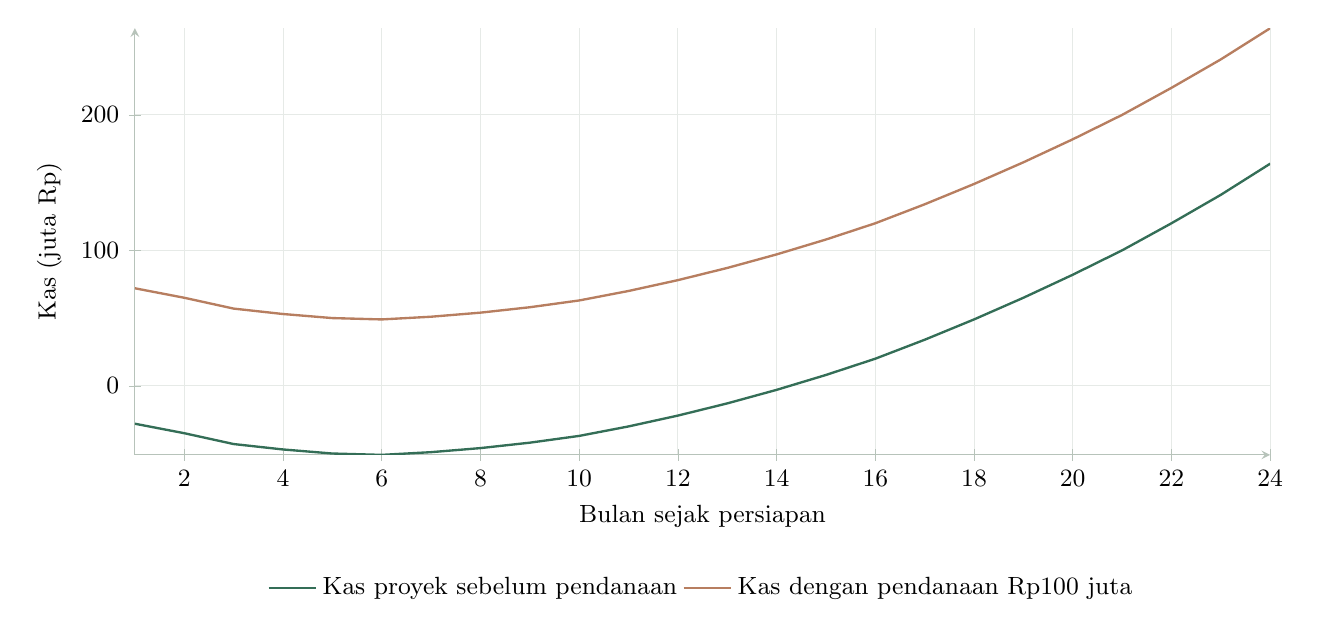
\begin{tikzpicture}\begin{axis}[width=16cm,height=7cm,scale only axis=false,
axis lines=left,axis line style={draw=rule},tick style={draw=rule},
tick label style={font=\small},label style={font=\small},
grid=major,grid style={draw=rule!35,line width=.3pt},
legend style={draw=none,fill=none,font=\small,at={(.5,-.26)},anchor=north},legend columns=-1,
xlabel={Bulan sejak persiapan},ylabel={Kas (juta Rp)},]
\addplot+[mark=none,color=forest,line width=.85pt] coordinates {(1,-28) (2,-35) (3,-43) (4,-47) (5,-50) (6,-51) (7,-49) (8,-46) (9,-42) (10,-37) (11,-30) (12,-22) (13,-13) (14,-3) (15,8) (16,20) (17,34) (18,49) (19,65) (20,82) (21,100) (22,120) (23,141) (24,164)};
\addlegendentry{Kas proyek sebelum pendanaan}
\addplot+[mark=none,color=clay,line width=.85pt] coordinates {(1,72) (2,65) (3,57) (4,53) (5,50) (6,49) (7,51) (8,54) (9,58) (10,63) (11,70) (12,78) (13,87) (14,97) (15,108) (16,120) (17,134) (18,149) (19,165) (20,182) (21,200) (22,220) (23,241) (24,264)};
\addlegendentry{Kas dengan pendanaan Rp100 juta}
\end{axis}\end{tikzpicture}
\end{document}
